%% 
%% Copyright 2007-2019 Elsevier Ltd
%% 
%% This file is part of the 'Elsarticle Bundle'.
%% ---------------------------------------------
%% 
%% It may be distributed under the conditions of the LaTeX Project Public
%% License, either version 1.2 of this license or (at your option) any
%% later version.  The latest version of this license is in
%%    http://www.latex-project.org/lppl.txt
%% and version 1.2 or later is part of all distributions of LaTeX
%% version 1999/12/01 or later.
%% 
%% The list of all files belonging to the 'Elsarticle Bundle' is
%% given in the file `manifest.txt'.
%% 
%% Template article for Elsevier's document class `elsarticle'
%% with harvard style bibliographic references

%\documentclass[preprint,12pt,authoryear]{elsarticle}

%% Use the option review to obtain double line spacing
%% \documentclass[authoryear,preprint,review,12pt]{elsarticle}

%% Use the options 1p,twocolumn; 3p; 3p,twocolumn; 5p; or 5p,twocolumn
%% for a journal layout:
%% \documentclass[final,1p,times,authoryear]{elsarticle}
%% \documentclass[final,1p,times,twocolumn,authoryear]{elsarticle}
%% \documentclass[final,3p,times,authoryear]{elsarticle}
\documentclass[final,3p,times,twocolumn,numbers]{elsarticle}
%% \documentclass[final,5p,times,authoryear]{elsarticle}
%% \documentclass[final,5p,times,twocolumn,authoryear]{elsarticle}

%% For including figures, graphicx.sty has been loaded in
%% elsarticle.cls. If you prefer to use the old commands
%% please give \usepackage{epsfig}

%% The amssymb package provides various useful mathematical symbols
\usepackage{amssymb}
%% The amsthm package provides extended theorem environments
\usepackage{amsthm}
\usepackage{amsmath}
\usepackage{mathtools}

\usepackage{mhchem}
\usepackage{xcolor}
\usepackage{csvsimple,booktabs}


\usepackage{algorithm}
\usepackage{algorithmicx}
\usepackage{algpseudocode}

%% The lineno packages adds line numbers. Start line numbering with
%% \begin{linenumbers}, end it with \end{linenumbers}. Or switch it on
%% for the whole article with \linenumbers.
%% \usepackage{lineno}

\journal{Sustainable Computing: Informatics and Systems}

\begin{document}

\begin{frontmatter}

%% Title, authors and addresses

%% use the tnoteref command within \title for footnotes;
%% use the tnotetext command for theassociated footnote;
%% use the fnref command within \author or \address for footnotes;
%% use the fntext command for theassociated footnote;
%% use the corref command within \author for corresponding author footnotes;
%% use the cortext command for theassociated footnote;
%% use the ead command for the email address,
%% and the form \ead[url] for the home page:
 \title{The impact of online machine-learning methods on long-term investment decisions and generator utilization in electricity markets}
% \tnotetext[label1]{}
 \author{Alexander J. M. Kell}
 \ead{a.kell2@newcastle.ac.uk}
% \ead[url]{home page}
% \fntext[label2]{}
% \cortext[cor1]{}
% \address{Address\fnref{label3}}
% \fntext[label3]{}

%\title{Validating a long-term electricity market model}

%% use optional labels to link authors explicitly to addresses:
%% \author[label1,label2]{}
%% \address[label1]{}
%% \address[label2]{}

\author{A. Stephen McGough, Matthew Forshaw}

\address{School of Computing, Newcastle University, Newcastle-upon-Tyne, United Kingdom}

\begin{abstract}
%% Text of abstract

\end{abstract}
%
%%%Graphical abstract
%\begin{graphicalabstract}
%
\includegraphics{grabs}
%Hello test
%\end{graphicalabstract}
%
%%%Research highlights
%\begin{highlights}
%\item Validating a model
%\item Optimisation
%\item Scenario modelling
%\end{highlights}

\begin{keyword}
%% keywords here, in the form: keyword \sep keyword
Long-Term Energy Modelling \sep Online learning \sep Machine learning \sep Market investment \sep Climate Change
%% PACS codes here, in the form: \PACS code \sep code

%% MSC codes here, in the form: \MSC code \sep code
%% or \MSC[2008] code \sep code (2000 is the default)

\end{keyword}

\end{frontmatter}

%% \linenumbers

%% main text
\section{Introduction}
\label{sec:intro}

The integration of higher proportions of intermittent renewable energy sources (IRES) in the smart grid will mean that the forecasting of electricity demand will become increasingly important. This is due to the fact that supply must mean demand at all times and that IRES are less predictable than dispatchable energy sources such as coal and combined-cycle gas turbines (CCGTs) \cite{Lu1993}.

Typically, peaker plants, such as reciprocal gas engines, are used to fill fluctuations in demand, that had not been previously planned for. These peaker plants are typically expensive to run and have higher greenhouse gas emissions than their non-peaker counterparts \cite{Mahmood2014}. 

To reduce reliance on peaker plants, it is helpful to know how much electricity demand there will be in the future so that more efficient plants can be used to meet this demand. To aid in this, machine learning and statistical techniques have been used to accurately predict demand based on several different factors and data sources, such as weather, day of the week and holidays \cite{Kell2018a, Al-Musaylh2018, Vrablecova2017, Hong2014}. 

%- Why the current approaches / systems don't solve the problem


While various studies have looked at how to predict electricity demand at various time horizons with the highest accuracy \cite{Singh2012}, the impact that the differing methods used have on a long-term electricity market has been studied to a lesser degree. In this paper, we compare several machine learning and statistical techniques to forecast 24 hours ahead to simulate a day-ahead market. 

In addition to this, we use the long-term agent-based model, ElecSim \cite{Kell, Kell2020}, to simulate the impact of different forecasting methods on long-term investments, power plant usage and carbon emissions from the year 2018 to 2035 in the United Kingdom. 


%- What is the innovation in this work

To compare the impact of different methods, we trial both online and offline machine learning and statistical techniques. Online learning methods can learn from novel data while maintaining what was learnt from previous data. This type of statistical modelling is useful for non-stationary datasets, and time-series data where recalculation of a model would take a prohibitive amount of time. We trial different algorithms and split times of the year into seasons, weekdays, weekends and holidays.

%- A short description of the solution


Using these methods, we take the error distributions, or residuals, and fit a variety of distributions. The distribution that best fits the respective residuals is then used and sampled from to adjust the demand in the model ElecSim. We then observe the differences in carbon emissions, and power plants invested in and utilised with each of the different statistical and machine learning methods to a base case.




%- What are the key take-home messages

We show that online learning has a significant impact on reducing the error for predicting electricity consumption a day ahead when compared to traditional offline learning techniques.

We show that the forecasting algorithm has a non-negligible effect on carbon emissions and use of coal, onshore, photovoltaics, reciprocal gas engines and CCGT. Specifically, the amount of coal, photovoltaics, and reciprocal gas used from 2018 to 2035 was proportional to the median absolute error, while both onshore and offshore wind are inversely proportional to the median absolute error.

Total investments in coal, offshore and photovoltaics are proportional to the median absolute error, while investments in CCGT, onshore and reciprocal gas engines inversely proportional.



%- Outline of the rest of the work

In Section \ref{sec:lit-review} we review the literature. We introduce the model ElecSim, and the methods used in Section \ref{sec:material}. The Methods section is shown in Section \ref{sec:methods}, results in Section \ref{sec:results}. We discuss and conclude our work in Sections \ref{sec:discussion} and \ref{sec:conclusion} respectively.

\section{Literature Review}
\label{sec:lit-review}

Multiple papers have looked at demand-side forecasting \cite{Singh2012}. These include both artificial intelligence \cite{Kim2000, Tiong2008,Quilumba2014} and statistical techniques \cite{Nazarko2005ARIMAApproach,Huang2003,Nguyen2017}. However, the impact of online learning has been discussed with less frequency. In addition to this, our research shows the impact of different algorithms on investments made, electricity sources contribution and carbon emissions over a 17 year period using the long-term electricity market agent-based model, ElecSim.

The have been several studies in diverse applications on the use of online machine learning to predict time-series data. Johansson \textit{et al}. apply online machine learning algorithms for heat demand forecasting \cite{Johansson2017}. They find that their demand predictions display robust behaviour within acceptable error margins. They find that artificial neural networks (ANNs) provide the best forecasting ability of the standard algorithms and can handle data outside of the training set.

Baram \textit{et al.} combine an ensemble of active learners by developing an active-learning master algorithm \cite{Baram2003}. To achieve this, they propose a simple maximum entropy criterion that provides effective estimates in realistic settings. Their active-learning master algorithm is empirically shown to, in some cases, outperform the best algorithm in the ensemble on a range of classification problems.

An extension of the FLORA algorithm is proposed by Schmitt \textit{et al} in \cite{Schmitt2008}. Their FLORA-MC enhances the FLORA algorithm for multi-classification and numerical input values. They use this algorithm for an ambient computing application. Ambient computing is where computing and communication merges into every day life. They find that their model outperforms traditional offline learners by orders of magnitude.

Pindoriya \textit{et al}. trial a number of different machine learning methods such an adaptive wavelet neural network (AWNN). They find that AWNN has good prediction properties when compared to other forecasting techniques such as wavelet-ARIMA, multi-layer perceptron (MLP) and radial basis function (RBF) neural networks as well as the fuzzy neural network (FNN).


Goncalves Da Silva \textit{et al}. show the effect of prediction accuracy on local electricity markets \cite{GoncalvesDaSilva2014}. To this end, they compare forecasting of groups of consumers in comparison to single individuals. They trial the use of the Seasonal-Naïve and Holt-Winters algorithms and look at the effect that he errors have on trading in an intra-day electricity market of consumers and prosumers. They found that with a photovoltaic penetration of 50\%, over 10\% of the total generation capacity was uncapitalised and roughly 10, 25 and 28\% of the total traded volume were unnecessary buys, demand imbalances and unnecessary sells respectively. This represents energy that the participant has no control.



\section{Material}
\label{sec:material}

\subsection{Machine Learning}

Machine learning is a methodology for finding and describing structural patterns in data \cite{Witten2011}. Typically machine learning algorithms are algorithms which are trained using data. These generate models which can make predictions or decisions with regards to classification of data \cite{Johansson2017}. Machine learning algorithms can be used for both static datasets as well as streaming data.




\subsection{Online learning}

Online machine learning is an extension of machine learning algorithms, that can be used on dynamic datasets, such as time-series data. In traditional machine learning algorithms, when new data is obtained, the historical data must be used to retrain the entire model with new model. This can be costly both in terms of time and in computation power \cite{Li2016}. Online algorithms therefore  avoids the repeated retraining of data and improves the learning efficiency \cite{Rong2009}.

Examples of such algorithms are Passive Aggressive Regressor \cite{Gzik2014}, Linear Regression, Box-Cox Regressor \cite{Box1964}, K-Neighbors Regressor \cite{forgy65}, Softmax Regression, Multilayer perceptron regressor \cite{Hinton1989}. For our work, we trial the stated algorithms, in addition to a host of offline learning techniques. The online techniques trialled were Lasso regression \cite{Tibshirani1996a}, ridge regression \cite{GeladiPaul1994Mrac},  Elastic Net \cite{Geostatistics2010}, least angle regression \cite{Fike1988}, Extra Trees Regressor \cite{Fike1988}, Random Forest Regressor \cite{Breiman2001}, AdaBoost Regressor \cite{Freund1997}, Gradient Boosting Regressor \cite{316}, Support vector regression \cite{Cortes1995}, and offline versions of Multilayer perceptron regressor, K-Neighbors regressor, linear regression.

We trial the previously mentioned statistical and machine learning algorithms, and vary the parameters using grid search and cross-validation in the python package, scikit learn \cite{scikit-learn}.

\subsection{Algorithms}

In this section we give a brief outline of the most successful online learning algorithms in this work.

\subsubsection{Multilayer perceptron}


\begin{figure}
	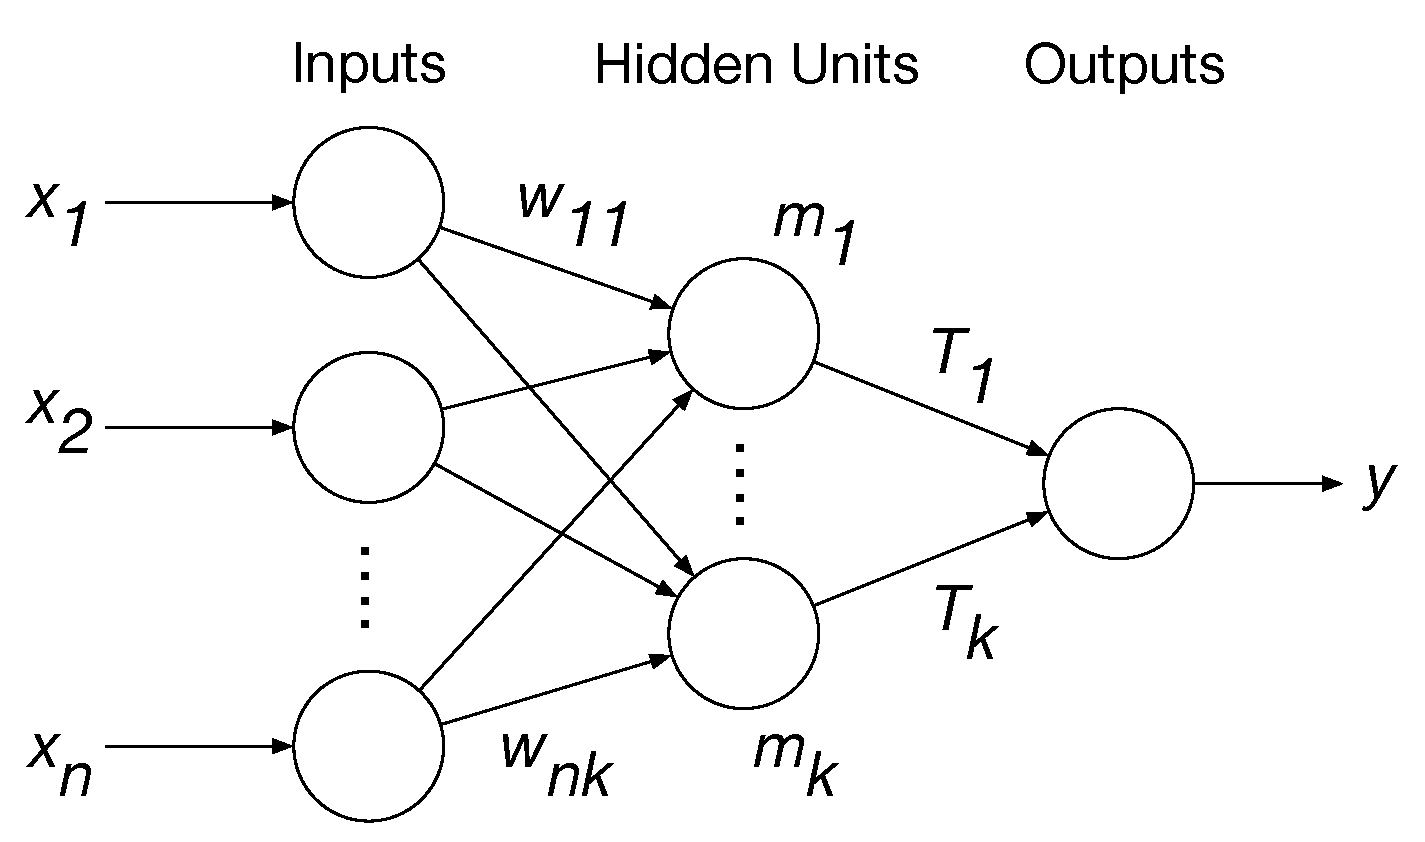
\includegraphics[width=0.4\textwidth]{figures/methods/Kell_eEnergy_Fig1.eps}
	\caption{A three layer feed forward neural network.}
	\label{fig:mlp}
\end{figure}

Artificial Neural Networks are a type of model which allow for non-linear relationships to be modeled between the input and output data \cite{Akaike1974}. A popular neural network is a feed forward multilayer network. Fig. \ref{fig:mlp} shows a three layer feed forward neural network with a single output unit, \textit{k} hidden units, $n$ input units. $w_{ij}$ is the connection weight from the $i$th input unit to the $j$th hidden unit,  and $T_j$ is the connecting weight from the $j$th hidden unit to the output unit \cite{Pao2007}. These weights transform the input variables in the first layer to the output variable in the final layer based upon the training data. 

Typically, a dataset is split into three sections, the test set, training set and validation set. The training set is used to find the connection weights of the network, whilst the test set is used to determine the accuracy of the models. The validation set allows for an unbiased evaluation of the model whilst tuning the hyperparameters, and can avoid overfitting by stopping training if the error begins to increase.

For a univariate time series forecasting problem, suppose we have N observations $y_1, y_2, \ldots, y_N$ in the training set, 
\begin{equation}
y_{N+1}, y_{N+2}, \ldots, y_{N+m}
\end{equation}
\noindent in the test set and we are required to predict \textit{m} periods ahead \cite{Pao2007}. 

The training patterns are as follows:
\begin{align}
y_{p+m} & =f(y_p, y_{p-1},\ldots,y_1)\\
y_{p+m+1} & =f(y_{p+1}, y_{p},\ldots,y_2)\\
&\vdotswithin  \notag \\
y_{N} & =f(y_{N-m},y_{N-m-1},\ldots,y_{N-m-p+1})
\end{align}

\noindent where $f$ is the function made up of weights and activation functions in the trained neural network.

The $m$ testing patterns are 

\begin{align}
y_{N+1} & =f(y_{N+1-m}, y_{N-m},\ldots,y_{N-m-p+2})\\
y_{N+2} & =f(y_{N+2-m}, y_{N-m+1},\ldots,y_{N-m-p+3})\\
&\vdotswithin  \notag \\
y_{N+m} & =f(y_{N},y_{N-1},\ldots,y_{N-p+1})
\end{align}

The training objective is to minimize the overall predictive error means (SSE) by adjusting the connection weights. For this network structure the SSE can be written as:
\begin{equation}
SSE = \sum_{i=p+m}^N(y_i-\hat{y}_i)
\end{equation}

\noindent where $\hat{y}_i$ is the output from the network. The number of input nodes corresponds to the number of lagged observations. Having too few or too many input nodes can affect the predictive ability of the neural network \cite{Pao2007}.

\subsubsection{Box-Cox regressor}

The ordinary least squares regression assumes normal distribution of residuals. However, when this is not the case the Box-Cox Regression may be useful \cite{Box1964}. It transforms the dependent variable using the Box-Cox Transformation fnction, and employs maxium likelihood estimatino to determine the optimal level of the power parameter lambda. The Box-Cox Regression requires that no dependent variable has any negative values.

Variable selection and ordinary least qquares output diagogues are identical to that of linear regression. 

The Box-Cox regression will transform the dependent variable as follows:

\begin{equation}
	y^{(\lambda)} = \frac{y^{\lambda}-1}{\lambda}\:if\:\lambda\neq0
\end{equation}
\begin{equation}
	y^{(\lambda)} = Ln(y)\; if\: \lambda=0
\end{equation}

and determine the optimal value of lambda by maximising the following log-likelihood function:

\begin{equation}
	L^{(\lambda)}=-\frac{n}{2}Ln(\hat{\sigma}^2_{(\lambda)}+(\lambda - 1)\sum_{i=1}^nLn(y_i)
\end{equation}

\noindent where $\hat{\sigma}^2_{(\lambda)}$ is the estimate of the least squares variance using the transformed y variable. 

\subsubsection{Passive-Aggressive regressor}

The goal of the Passive-Aggressive (PA) algorithm is to change the model as little as possible to correct for any mistakes and low-confidence predictions it encounters \cite{Gzik2014}. Specficially, with each example PA solves the following optimisation \cite{Ma2009}:

\begin{align}
	\boldsymbol{w}_{t+1}\leftarrow argmin \frac{1}{2}\left|\left|{\boldsymbol{w}_t-\boldsymbol{w}}\right|\right|^2 \\
	s.t. \; \; y_i(\boldsymbol{w}\cdot \boldsymbol{x}_t)\geq1.
\end{align}

\noindent Updates occur when the inner product does not exceed a fixed confidence margin - i.e., $y_i(\boldsymbol{w}\cdot \boldsymbol{x}_t)\geq1$. The closed-form update for all examples is as follows:
\begin{equation}
	\boldsymbol{w}_{t+1}\leftarrow \boldsymbol{w}_{t} + \alpha_t y_t \boldsymbol{x}_t
\end{equation}

\noindent where $\alpha_t=max\left\{\frac{1-y_t(\boldsymbol{w}_t\cdot\boldsymbol{x}_t)}{\left|\left|\boldsymbol{x}_t\right|\right|^2},0\right\}$. Full details of the derivation can be found in \cite{Gzik2014}.

\subsection{Long-term Energy Market Model}


In order to evaluate the different carbon strategies we used the model developed by Kell \textit{et al}., ElecSim \cite{Kell,Kell2020}. ElecSim is an agent-based model which mimics the behaviour of decentralised electricity markets. For this paper, we have parametrised the model to data for the UK in 2018 to act as a digital twin of the UK electricity market. This includes the power plants in operation in 2018, and the funds available to their respective companies \cite{dukes_511, companies_house}.

Six fundamental sections make up ElecSim: 1) power plant data; 2) scenario data; 3) the time-steps of the algorithm; 4) the power exchange; 5) the investment algorithm and 6) the generation companies (GenCos) as agents. ElecSim uses a subset of representative days of electricity demand, solar irradiance and wind speed to approximate a full year. In this context, representative days are a subset of days which when scaled up can adequately represent a year. Figure \ref{fig:model_details} details how these components interact. 

Specifically, the configuration file details the scenario which can be set by the user. This includes electricity demand, carbon price and fuel prices. The data sources parametrise the digital twin to a particular country, including information such as wind capacity and power plants in operation. Generation Companies own and invest in power plants. These power plants are then matched to electricity demand using a spot market.



\begin{figure}
	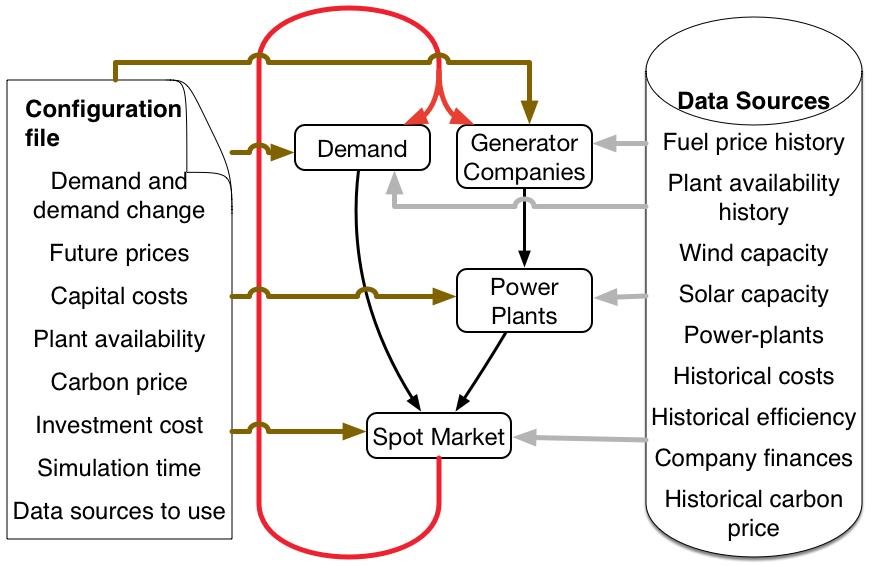
\includegraphics[width=0.48\textwidth,natwidth=610,natheight=400]{figures/methods/System_overview_large.png}
	\caption{System overview of ElecSim \cite{Kell}.}
	\label{fig:model_details}
\end{figure}


The market runs in merit-order dispatch and bids are made by the power plant's short-run marginal cost (SRMC). Investment in power plants are based upon a net present value (NPV) calculation. NPV is able to evaluate and compare investments with cash flows spread over many years. This is shown formally in Equation \ref{eq:npv_eq}, where $t$ is the year of the cash flow, $i$ is the discount rate, $N$ is the total number of years, or lifetime of power plant, and $R_t$ is the net cash flow of the year $t$:
\begin{equation} \label{eq:npv_eq}
NPV(t, N) = \sum_{t=0}^{N}\frac{R_t}{(1+t)^t}.
\end{equation}
The yearly income for each power plant is estimated for each generation company by running a merit-order dispatch electricity market 10 years into the future. However, the expected cost of electricity 10 years into the future is uncertain. We therefore use the reference scenario projected by BEIS and use the predicted costs of electricity calibrated by Kell \textit{et al} \cite{DBEIS2019, Kell2020}. The agents predict the future carbon price by using a linear regression model.


 
\section{Methods}
\label{sec:methods}

- Use of hyperparameter tuning, talk about time taken to train/query models.\\
- Talk about ML methods used\\
- Talk about residuals\\
- Talk about sampling from residuals and placing these errors on the day-ahead market.\\


\section{Results}
\label{sec:results}

- Results of offline learning, online machine learning shown. Include residuals and MAE,MAPE,MASE etc\\

- Results of the residuals on the output of ElecSim until 2035.\\

\section{Discussion}
\label{sec:discussion}

- Discuss the impact of this on the electricity market and global economy. Make suggestions.

\section{Conclusion}
\label{sec:conclusion}

- Summary of work and future work.

\section{Funding Sources}

This work was supported by the Engineering and Physical Sciences Research Council, Centre for Doctoral Training in Cloud Computing for Big Data [grant number EP/L015358/1].





%% The Appendices part is started with the command \appendix;
%% appendix sections are then done as normal sections
%% \appendix

%% \section{}
%% \label{}

%% If you have bibdatabase file and want bibtex to generate the
%% bibitems, please use
%%
  \bibliographystyle{elsarticle-num} 
  \section*{References}
  \bibliography{library,bib_custom}

%% else use the following coding to input the bibitems directly in the
%% TeX file.

%\begin{thebibliography}{00}
%
%%% \bibitem[Author(year)]{label}
%%% Text of bibliographic item
%
%\bibitem[ ()]{}
%
%\end{thebibliography}
\end{document}

\endinput
%%
%% End of file `elsarticle-template-harv.tex'.
	